


\section{Geology of Migovec}

\subsection{The Julian Alps}
\label{sec:The Julian Alps}

\paragraph{Geography} 
\label{par:Geography} 
\passage{Tolminski Migovec} belong to the \passage{Julian Alps}, in the easternmost sector of the \passage{Southern Alps} \citep{bavec2004late}. 
They \passage{Julian Alps} are bounded by the Pannonian and  Fruili-Veneto bassins to the east and west respectively, while to the north, they are separated from the \passage{Eastern Alps} by the Periadriatic lineament\fref{map:geol large scale}. Southward from the South Alpine front, they become the \passage{Dinarides} \citep{placer1998contribution,burrato2008sources}.
This carbonate dominated massif is characterised by high relief with valley floors located 100-400m asl and peaks in excess of 2000m asl  \citep{vsmuc2009tectonic}. Relief production is attributed to both tectonic processes and glaciation, and \citet{vsmuc2009tectonic} argue for the primacy of the litho-sructural setting for the observed meso (1-10m) and macro- (100-1000m) scale relief.


\paragraph{Structural style}
\label{par:Structural style}
Overall, the tectono-stratigraphic setting \sidenote{The interplay between relief generation, erosion and sedimentary deposition during \emph{orogenesis} or moutain building events} of the \passage{Julian Alps} is a result of continued northward motion (about 2mm.a$^{-1}$ \citep{burrato2008sources} and since the Miocene,  counter-clockwise rotation of the Adriatic microplate \citep{marton2003palaeomagnetic}. 
The convergence of the Adria microplate with the Eurasian plate is quantitatively described by GPS velocity fields \citep{grenerczy2005tectonic}. 
Such convergence was led to the formation of Alpine and Dinaric mountain chains, and still generates earthquakes today ($M_w$ > 5) in the brittle deformation zone.

Slovenia, and in particular the area north east of Tolmin are located in the north-eastern corner of the Adria-Europe collisional belt. 
This area, at the critical juncture between the Alpine and Dinaric chains overlook rim of high topography around the relatively rigid, undeformed Adria microplate, which is only exposed in the Istria peninsula \citep{vsmuc2009tectonic}. 
It is buried under a thick cover of foredeep \sidenote{Foredeep basins form in the immediate vicinity of collisional belt as thickened crust deforms the somewhat elastic plate underneath, creating a trough where the material sourced from the nearby mountains is preferentially deposited}sediments in the Friuli-Venetian plain. 

It is useful to define a hierarchy for the subdivision of tectonic units within the Tolmin area. 
At first order, the \passage{Southern Alps} lie between by the Periadriatic lineament and South Alpine front \citep{placer1998contribution}. 
Second order units, e.g. the Zlatna, Julian (locally Krn) and Tolmin nappes are slices bounded by south verging thrust faults. 
This reverse thrusting resulted in an inversion of stratigraphical order, and place massive upper Triassic limestones at the top of the sequence, while the Jurassic/Cretaceous marls and limestones of the Tolmin nappe crop out at much lower elevation.

\begin{map}[b!]
\checkoddpage \ifoddpage \forcerectofloat \else \forceversofloat \fi
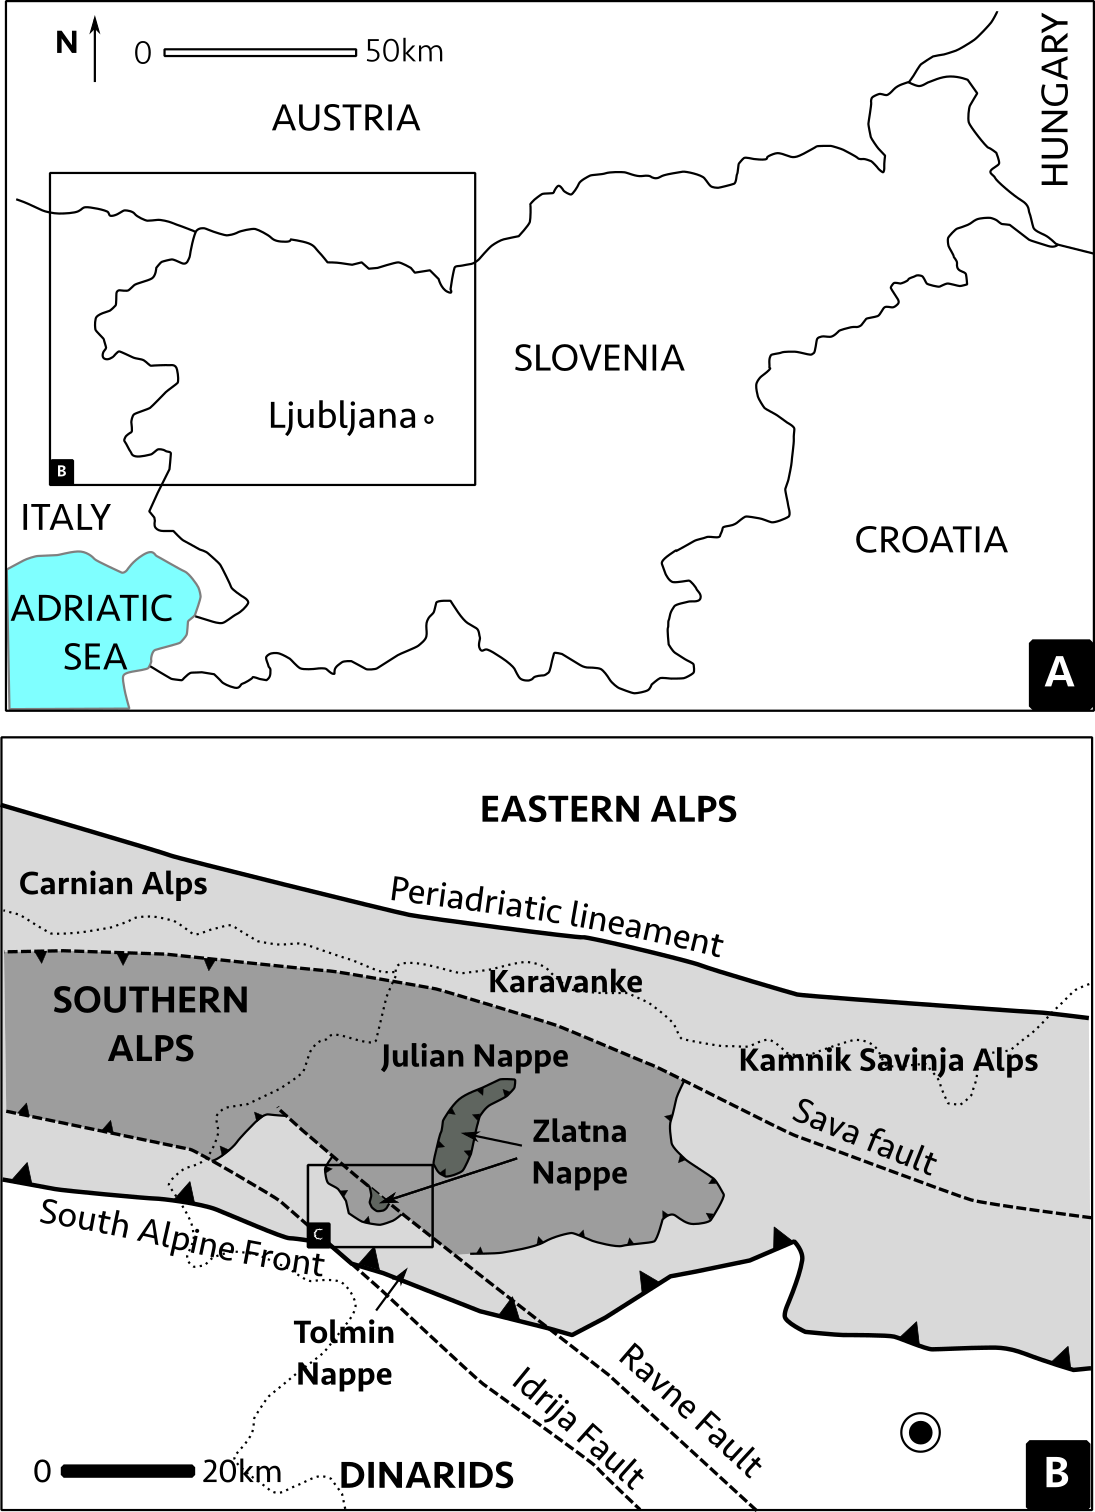
\includegraphics[width = \textwidth]{images/maps-of-mig/geology_large.png}
\caption[Structural setting of NW Slovenia]{\emph{(a)} Overview map of Slovenia \emph{(b)} The structural setting of northwestern Slovenia shows the \protect\passage{Tolmin} area straddling the active \protect\passage[fault]{Idrija} and \protect\passage[fault]{Ravne} faults. The \protect\passage{Migovec System} is developed within the Slatna overthrust and the underlying Dachtsein limestone, as shown in the geological map from \citet{buser1986tolmavc}. Figure modified from \citet{vsmuc2009tectonic}}
\label{map:geol large scale}
\end{map}


 
\paragraph{Alpine deformation}
\label{par:alpine deformation}
That the \passage{Julian Nappe}, which comprises the cave forming Dachstein Limestones of the \passage{Krn}-\passage{Migovec} area was transported towards the south during the Alpine orogen is commonplace in the litterature \citep{doglioni1987eoalpine,placer1998contribution}. 
The weak and easily deformed Carboniferous clastics basement of the \passage{Julian Alps} provided a detachment horizon along which the nappe was transported from the north southwards. The question of the timing of transport of this nappe is somewhat more difficult. \citet{buser1986tolmavc} attributes a Neogene (~23Ma to 3Ma BP) age to this tectonic structure, while \citet{placer1998contribution} argues it could be slightly older, starting in mid to Late Oligocene (28Ma BP).

\paragraph{Present day stress regime}
\label{par:present day stress regime}
The activity on this heavily faulted boundary between Adria and Eurasia is highlighted by recent destructive earthquakes: $M_w$=6.4 on the Italian side in 1976 \citep{pondrelli2001seismotectonic}, and $M_w$=5.7 and $M_w$=5.2 on the Slovenian side in 1998 \citep{bajc20011998} and 2004 \citep{aoudia2005july} respectively. 
To highlight the vulnerability of this region, it is also worth keeping in mind that the largest earthquake ever at this junction between the \passage{Southern Alps} and the \passage{Dinarides} was the 1511 western Slovenia earthquake ($M_w$= 6.8). It is believed to have resulted in at least 12,000 deaths \citep{fitzko2005constraints}.
Fault plane solutions for the many $M_w$=4-6 regional quakes demonstrate that the mode of deformation on the Italian side is chiefly by thrusting \citep{poli2002new}, while deformation is accommodated by dextral slip on the Slovenian side \citep{poljak2000seismotectonic}. 
The main strike-slip faults in NW Slovenia i.e. the \passage[fault]{Idrija}, \passage[fault]{Ravne} and \passage[fault]{Sava} faults from south to north have a spectacular topographic expression. 

Indeed, the \passage[fault]{Ravne} and \passage[fault]{Idrija} faults' expression was mapped by \citet{cunningham2006application} with the aid of LiDAR data. The \passage[fault]{Ravne} fault is ~35km long, yet seismic source modelling suggests a 13km only segment was involved in the 1998 earthquake, therefore it is possible that this fault generated stronger earthquakes in the past; it is thought it was involved in the devastating 1511 earthquake \citet{fitzko2005constraints}.
On the following geological map \fref{map:mapofgeology} the NW-SE trending fault passes to the NE of \passage{Krn}, between \passage{Gru\v{s}nica} and \passage{Tolminski Migovec} and heads towards \passage{Tolminske Ravne} hamlet.

Crucially, the Ravne fault segments pass through the \passage{Tolminka} springs basin, and its Quaternary (3Ma to Present) activity has played a primary role in the building local topography of the Tolminka valley (±1200m relief), which is described as a small pull-apart basin \citet{cunningham2006application}. 
In short this basin highlights the interplay between old Alpine structures, recent cross-cutting faults, glacial and hillslope erosional processes and karst development.

\paragraph{Summary of tectonic history}
\label{par:summary of tectonic}
\citet{vsmuc2009tectonic} recognise two main landscape building tectonic events in the area of the Triglav lakes valley, located just 10km to the east of \passage{Tolminski Migovec}.

\begin{citemize}
\item The transport of the Mesozoic carbonate platforms which form the \passage{Julian Alps} as described by \citet{placer1998contribution} and \citet{buser1986tolmavc} from possibly mid-Oligocene to mid-Miocene. This resulted in the various south verging overthrusts of the Zlatna and Julian nappes and the building of the topography like the Zelenacia ridge in the Triglav lakes valley. The resulting compressional tectonic structures are mostly E-W oriented.
\item Neogene strike-slip faulting cross-cutting the Alpine generated topography, producing youthful landforms \citep{vsmuc2009tectonic,cunningham2006application} such as the Tolminka Springs Basin, continuing today, highlighted by earthquake activity. These NW-SE oriented faults cross-cut the previous Alpine structures.
\end{citemize}

 \begin{map*}[t!]
 \checkoddpage \ifoddpage \forcerectofloat \else \forceversofloat \fi
\centering
  \includegraphics[width=\textwidth]{"images/maps-of-mig/geological_map_with_symbols".png}
  
  \caption{Geological map of the Tolmin Area, modified after \citet{buser1986tolmavc}}
  \label{map:mapofgeology}
 \end{map*}

\subsection{Landscape development and controls}
\paragraph{Lithology}
\label{par:lithology}
\marginnote{Lithology is described as summary of the gross characteristics of a rock}

\passage{Tolminski Migovec} is mainly formed by a sequence of massive to well-bedded (1-3m) pure grey to buff limestones with patches of dolomite \citep{buser1986tolmavc} belonging to the Dachstein formation (in Slovene 'Dachteinski apnenec'), which derives its name from the Dachstein massif near Salzburg, Austria \citep{ogorelec1996dachstein}. 


The rock formed during the Upper Triassic Norian to Rhaetian age (228 -101.3 Ma) and now forms the backbone the \passage[Calcareous Alps]{Southern Calcareous Alps} \citep{bosellini1974triassic} and crops out all over the \passage{Northern Calcareous Alps} \citep{fischer1975tidal,schwarzacher2005stratification}. It has given rise to spectacular landscapes spread over Southern Europe, from Hungary \citep{haas2004characteristics} to Sicily \citep{catalano1974ciclotemi}.
Its ubiquity has wide ranging implications for the palaeogeography of this region in Norian to Rhaetian times.

The Dachstein limestone is typically well-bedded, nearly 1km thick and comprises both karst and palaeokarst phenomena \citep{ogorelec1996dachstein,haas2007characteristics}. Locally, it is underlain by the equally extensive Main Dolomite (in German 'Hauptdolomit'). The dachstein formation is thought to have been deposited in quiet but thriving shallow marine environments, where the accumulation of biogenic calcareous material was compensated by the steady sinking of the carbonate platform. 

Debate is ongoing as to the origin of the cyclic pattern of the limestone beds often called \emph{Lofer cyclothems} --- so named after the Lofer locality in Austria where they were first described. 
These cyclothems were identified and interpreted by \citet{fisher1964lofer} as cyclic sequences tracking deepening upwards depositional environments.
The idealised cyclothem model shows three groups A, B, C corresponding to  subaerial, tidal and subtidal deposition environments respectively.  

This is demonstrated by palaeokarst solution vugs, the presence of argillaceous --- here terrestrially derived --- and often iron oxide rich residues and evidence of subaerial weathering, even palaeokarst in Group A.

Group B is often characterised by the presence of dessication cracks, partial dolomitisation; it is often laterally discontinuous, with variable thicknesses (5-155cm).

Group C, often the most abundant, comprises wackestones (rich in carbonatic mud) and packstones (dominated by biogenic fragments).


Often, the measured sections differ from the ideal model by the absence of certain members of the sequence. Indeed compared with the Dachstein limestones deposited in the Dinaric range, the limestones of the Krn area show more numerous and more pronounced periods of emersion \citep{ogorelec1996dachstein}.

 With some authors favouring local tectonic control as a causal mechanism  for relative changes in sea level \citep{goldhammer1990depositional,enos1998lofer}, others \citep{fisher1964lofer,balog1997shallow,haas2004characteristics,doi:10.1130/G21578.1}, prefer orbitally forced environmental fluctuations such as \emph{Milankovitch cycles} which result from periodic fluctuations in solar insolation linked with the Earth's \emph{precession}, \emph{tilt} and \emph{ellipticity} cycles. 

 \paragraph{Glacial landforms}
 \citet{bavec2004late} used a combination of geological mapping and dating the identified glacial deposits in order to constrain the extent of late Quaternary glaciation in the upper So\v{c}a valley, which is relevant to the Tolmin area.

 Most notably, they find no clearly expressed glacial geomorphic features downstream of the town of Bovec; on the contrary, all landforms such as end moraines or glacial cirques are limited to the high reaches on the valleys. 

Locally, the bowl shaped hanging valley between the \passage{Migovec Plateau} and \passage{Vhr Nad \v{S}krbino} is one example of glacial cirque. Notably, the high resolution mapping of \citet{cunningham2006application} could not find any signes of side or -end moraine, nor any other glacially derived deposits within the \passage{Tolminka springs} basin and interpreted the sheer walls near \passage{Polog} as segments of the Ravne fault in a pull-apart basin. 
This is consistent with the view of \citet{vsmuc2009tectonic} on the relative primacy of tectonics over glacial processes on landscape building in the \passage{Triglav} area.


 \paragraph{Karst landscape}
Karst terrain arises from the combination of high rock solubility and well developed secondary fracture porosity \citep{ford2013karst}. 

Such terrains exhibit several key features: fluted outcrops, sinks, caves, springs, blind valleys etc... It is the present of an unusual hydrology which dictates the development of 'karstic landscapes'. 

These landforms are generated by the dissolution of rock along natural subterranean pathways provided by geological features (joint, bedding planes, faults), the principles of which have been described by \citet{dreybrodt1996principles}, under several numerical models.

It is now commonplace to think of inception horizons \citep{lowe1997carbonate} as promoting early cavern development and governing the maturation of a karst system. Soluble rocks with well developed primary or secondary porosities tend to support excellent karst. It comes as no surprise then that the well-bedded, often jointed and heavily faulted Dachstein limestones of Migovec exhibit most of the staples of alpine karst.

The development of karst is termed either \emph{eogenetic}, \emph{mesogenetic} or \emph{telogenetic} according to the following rules:
\begin{citemize}
\item dissolution of the host rock coeval with or immediately following its deposition and lithification is eogenetic karst 
\item dissolution of the rock by hypogene (deep seated) fluids as it is buried, is termed mesogenetic karst
\item dissolution of the rock by weakly acidic rainwater when the rock mass is made available by uplift is term telogenetic karst
\end{citemize}

The karst of \passage{Tolminski Migovec} shows both aspect of eogenetic karst such as solution vugs within \emph{Lofer cyclothems}, which developed during deposition and more significantly, telogenetic karst, which produced the many kilometres of enterable caves within the mountain.

The surface of the \passage{Migovec Plateau} is famously riddled with shakeholes and dolines. A cursory inspection of a topographic map shows that a majority of these 10-30m deep shakeholes are aligned with the dominant tectonic structures within the Migovec area (namely NNW to SSE lineaments). 

\subsection{The karst aquifer of Migovec} 
The karst aquifer is divided into two main zones: \begin{citemize} 
\item the \emph{phreatic} zone, which consists of a network of water-filled conduits, planes or matrix under hydrostatic pressure. The largest phreatic tunnels are accessible to divers, either from within the cave (at siphons or 'sumps') or a springs, where the water finished its underground course. It is generally the actively forming part of a cave system where fissures are enlarged by dissolution.
\item the \emph{vadose} zone, which consists of dry passages, deeply incised stream canyons or waterfall shaft series. These are accessible to non-diver speleologists and often contain sediment banks, \emph{speleothems}. Such passages are modified by the mechanical breakdown of the cave roofs, which generate large underground chambers or caverns.
\end{citemize}

The thickness of the vadose zone on Migovec, that is the elevation difference between the entrance and the sump level, is about 1km. The type of recharge present is diffuse autogenic and as such, water collects from innumerable fissures on the surface into small inlets. These cascade down over 15 identified shaft and canyon series (but there are probably more), often disappearing down immature underground canyons. 

In over 40 years of exploration, we have not found a master streamway, that is to say, a collector underground stream ending in a sump, whose resurgence is known. Rather, we have followed the disparate streams to at five different sumps located each within 30m of 890m. Other shallower siphons within the System are called 'perched', as they are presumably the sign of a local watertable.

\begin{pagefigure}
\checkoddpage \ifoddpage \forcerectofloat \else \forceversofloat \fi


\begin{subfigure}{\linewidth}
\centering
 \includegraphics[width=0.6\linewidth]{"images/maps-of-mig/rose_diagram".png}
\caption{}
 \label{fig:rose diagram}
 \end{subfigure}
 \vspace{3mm}
\begin{subfigure}{\linewidth}
\centering
 \includegraphics[width=0.6\linewidth]{"images/maps-of-mig/rose diagram 2".png}
 \label{fig:rose diagram 2}
 \caption{}
 \end{subfigure}
 
  \caption{A rose diagram depicting the azimuth ($\phi$) of cave passages. This was extracted from a .3d file produced on Survex, where  $n$ is the number of stations, $\theta$ is the inclination angle and the radial grid is the percentage fraction of passages falling in a specific orientation \emph{(a)} $n=5084$, $\theta <45°$ and \emph{(b)} $n=912$, $\theta \ge 45 \textdegree$. Each sector is 10\textdegree wide. Bin colour shows passage length distribution}
\end{pagefigure}

Reaching the 'water table' often occurs when the underground course of the water hits a lithological or tectonic boundary. In the case Migovec, it is probable that the contact between the Zlatna overthrust and the underlying Krn nappe, whose topmost rocks are relatively insoluble marls, will provide a benchmark for the watertable. It is curious to note however, that the five deep sumps occur above this impervious horizon - it means the sump level is likely the contact with a dolomitic body, which leaves open the possibility for further depth development. 

Imperial College Caving Club have attempted to trace the water from \passage{Sistem Migovec} \citep{hm1} to the \passage{Tolminka}, \passage{Zadla\v{z}\v{c}ica} and \passage{Sava} rivers.
 
 
 \subsection{Structural control of cave passage orientation}
 Horizontal sections of passage come under the name of \emph{galleries}: they are dry, fossil tubes which were enlarged when they were under the water table, and thus were part of the phreatic zone. Their orientation is guided by the intersection of bedding planes (near horizontal) and vertical joints and faults. They have a characteristic elliptical cross-section, which can be obscured by mechanical failure of the ceilings. Sometimes, sediment banks and speleothems are present (\fref{fig:atlantis}, \fref{fig:leprechaun}).

Under the assumption that survey legs are `optimised' \sidenote{ie:that they are the longest possible given passage geometry. This is almost always valid for two reasons: 1) stations are chosen to reduced the survey workload inside the cave; 2) excessive 'bouncing off the walls' adds artificial length to the cave and is therefore frowned upon} the orientation of near horizontal cave, and in particular that of long stretches of rectilinear passage appears to be non-random. 

While short survey legs (<$4m$), which are typical of short, twisting complex passage or breakdown are regularly distributed within the azimuth space, long survey legs >$8m$, and by extension long rectilinear cave passage are significantly more numerous in the $145-195\textdegree  \pmod{180\textdegree}$  sectors and to a lesser degree within the $35-55\textdegree   \pmod{180\textdegree }$ sector (\fref{fig:rose diagram}).

The orientation is therefore likely dictated by a set of planar discontinuities (joints or fractures) aligned with the general direction NNW-SSE, and a minor set in direction NE-SW \fref{fig:rose diagram}. This conclusion is in accord with in-cave observations \citep{hm1}  and previous surface mapping \citep{buser1986tolmavc} . Indeed many, if not all of the strike-slip and normal faults whose planes are chiefly vertical are oriented in a NNW-SSE direction and to a lesser extent in a NE-SW. (\fref{map:mapofgeology}).

At depth this also supported by observations on several abandoned phreatic routes and low gradient vadose canyons:
 
\begin{citemize} 
\item \passage{Minotaur Rift} (\fref{fig:minotaur_rift})
\item \passage{Amazing Grace} and \passage{Atlantis}  (\fref{fig:atlantis})
 \item \passage{Push Your Luck} - \passage{Agartha} (\fref{map:pushyourluck})
 \item \passage{Highway 32} (\fref{fig:highway32})
 \end{citemize} 

These passages are useful markers of the water table position in the past
 Vertical sections of passage are called \emph{pitch}, \emph{drop}, \emph{shaft}, \emph{pit} or \emph{pot}; in Slovene \emph{brezno}. 
 Several pitches in a row make a \emph{series}. Some ~15 pitch series in Migovec are over 200m deep, and most are over 400m.
Some of the deepest shafts within the system include \passage{Silos} (113m), \passage{Plopzilla} (105m), \passage{Happy Monday} (81m). They are commonly over 10m in diameter at the base. 

S 

\begin{marginfigure}
\checkoddpage \ifoddpage \forcerectofloat \else \forceversofloat \fi
\centering
 \frame{\includegraphics[width=\linewidth]{"images/maps-of-mig/marls_limestone".jpg}} 
 \caption{An example of the Jurassic marl and limestone succession, with pyrite nodules and minor fault offsetting the thick micritic limestone beds \pic{Tanguy Racine} on the \protect\passage{Slovenska Geolo\v{s}ka Pot}}
 \label{marls and limestones}
\end{marginfigure}

